\chapter{The Atmospheric Statistical Picture}\label{ch:statistical_picture}

In this chapter a method to build a \emph{statistical picture} of the
atmosphere is presented. First the ERA5 dataset is introduced: this
constitutes the set of statistical populations for the relevant meteorological
parameters that we have choosen to achieve this result; then the statistical
picture of the atmosphere is defined and the described in details; finally,
the mathematical objects we have used to describe expected daily and annual
variations of meteorological parameters at Pico del Teide are analyzed.

These results form the basis to get an estimate of the atmosphere
brightness temperature in the microwave range. This contribution, and its
seasonal variations as well, will be studied in the following chapters.

\section{The ERA5 Dataset}

As we have discussed in \autoref{ch:atm_model}, to calculate the extra load
caused by atmospheric effects, we must solve the radiative transfer equation
in the case of a dispersive medium at local thermodynamic equilibrium. The
solution depends on the physical properties of the medium. In particular,
it is determined by its physical temperature, $T$, and absorption
coefficient, $\alpha_\nu$. In turn, these quantities depends on a set a
meteorological parameters, which undergo seasonal variations.

In order to create a reliable statistical representation of these daily and
annual variations, we employed the ERA-5 dataset by the \emph{European
Centre for Medium-Range Weather Forecasts} (ECMWF). ECMWF uses forecast
models and data assimilation systems to \emph{reanalyse} archived
meteorological observations, creating global datasets describing the
recent history of the atmosphere, land surface, and oceans. In particular,
ERA5 provides hourly estimates of a large number of atmospheric, land and
oceanic climate variables. The data cover the whole Earth surface and
resolve the atmosphere using \num{137} levels from the surface up to a
height of \SI{80}{\kilo\meter}. ERA5 reanalysis relies on the \emph{Global
Circulation Model} (GCM) algorithm (McGuffie, Henderson-Sellers) making use
of the historical measures as forcing terms into GCM simulations to produce
data homogeneously gridded characterized by high spatial and temporal
resolution.

\autoref{fig:pwv_canary_islands} shows PWV distribution from ERA5 dataset
in Canary Island for the twelfth hour of the first day of the 1980. The
archipelago in covered by a grid of \num{30} by \num{30} \si{\kilo\meter}
\emph{pixels}  (\ang{0.25} by \ang{0.25} in geographic coordinate system).
As expected, precipitable water vapour takes its lowest values for
continental lands, its greatest values for pixels covering ocean and
intermediate values in correspondence of islands. \autoref{fig:pwv_tenerife}
focuses on Tenerife islands, showing that the whole site is covered by only four
pixels, which are delimited by a fuchsia perimeter in the figure.
In the following chapters we will prove that ERA5 spatial
resolution is in fact not enough to describe the specific meteorological
conditions at Pico del Teide, and at observation sites found on
small islands in general.

\begin{figure}
        \centering
        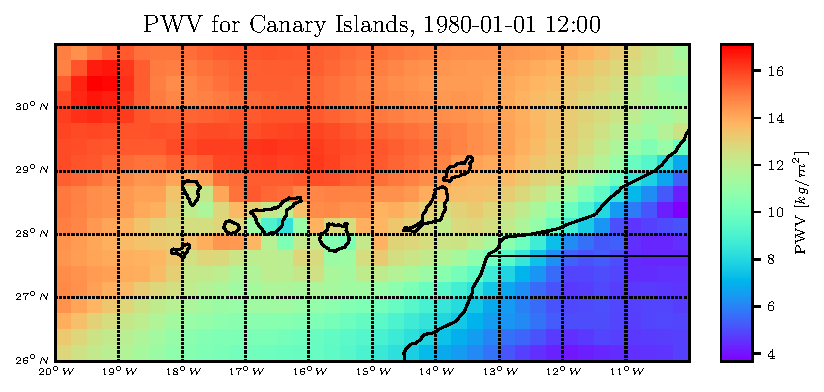
\includegraphics[width=\textwidth]{PWV_Canary_Islands_1980-01-01_12-00}
        \caption{PWV Canary Islands}
        \label{fig:pwv_canary_islands}
\end{figure}

\begin{figure}
        \centering
        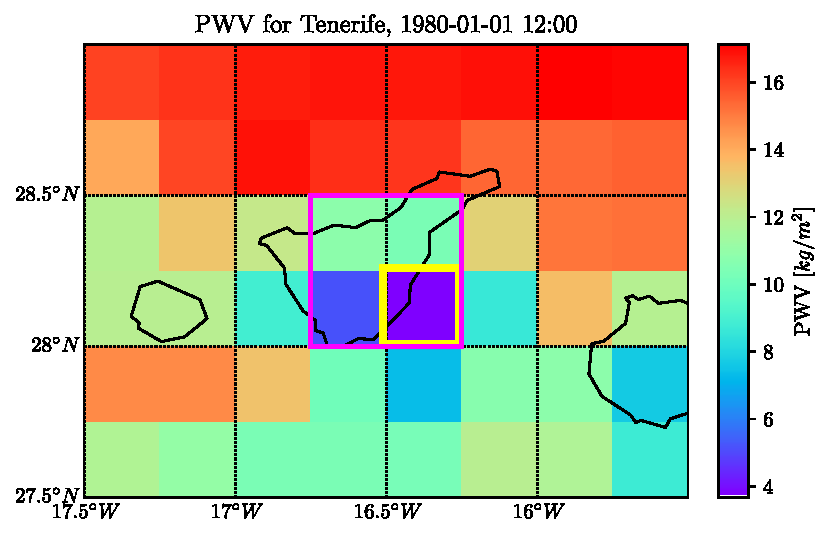
\includegraphics[width=\textwidth]{PWV_Tenerife_1980-01-01_12-00}
        \caption{PWV Tenerife}
        \label{fig:pwv_tenerife}
\end{figure}

\subsection{The Set of Relevant Meteorological Parameters}

Climate reanalysis data ranging from January the 1th 1979 to November
the 21th 2020 have been acquired by means of the ECMWF Web API, for a total of
\num{367200} hours in UTC. Downloaded data concern only one of the pixels found in
\autoref{fig:pwv_tenerife}: the one including the territory of Teide
observatory, which in the figure is enclosed by a yellow
square.

The relevant parameters, essential to provide a complete description of our
atmosphere, have been selected, for a total of seven quantities:

\begin{itemize}
        \item \textbf{total column cloud liquid water} (\textbf{tclw}):

        the amount of liquid water contained within cloud
        droplets in a column extending from the surface of the Earth to the
        top of the atmosphere, measure in \si{\kilo\gram\per\square\meter}.
        Rain water droplets, which are much larger
        in size (and mass), are not included in this parameter;

        \item \textbf{total column cloud ice water} (\textbf{tciw}):

        the amount of ice contained within clouds in a column extending
        from the surface of the Earth to the top of the atmosphere,
        measured in \si{\kilo\gram\per\square\meter}. Snow
        (aggregated ice crystals) is not included in this parameter;

        \item \textbf{total column water vapour} (\textbf{tcwv}) or \textbf{precipitable
        water vapour} (\textbf{PWV}):

        the total amount of water vapour in a column
        extending from the surface of the Earth to the top of the
        atmosphere, measured in \si{\kilo\gram\per\square\meter};

        \item \textbf{skin temperature} (\textbf{skt}):

        the temperature of the surface of the Earth, measured in
        \si{\kelvin};

        \item \textbf{surface pressure} (\textbf{sp}):

        the pressure of the atmosphere on the surface of land, sea and
        in-land water, measured in \si{\pascal};

        \item \textbf{10 meter temperature} (\textbf{T10M}):

        this parameter is not present in the ERA5 database, then it has
        been deduced from the \emph{2 meter temperature} (2t) parameter
        assuming a linear decrease in troposphere temperature of
        \SI{6.5e-3}{\kelvin\per\meter}. The 2t parameter represents the
        temperature of air at \SI{2}{\meter} above the surface of land, sea
        or in-land waters;

        \item \textbf{10 meter V wind component} (\textbf{10v}):

        the northward component of the 10m wind. It is the horizontal speed
        of air moving towards the north, at a height of ten meters above
        the surface of the Earth, measured in \si{\meter\per\second};

        \item \textbf{10 meter U wind component} (\textbf{10u}):

        like the latter parameter, but for the eastward component of the
        wind speed.
\end{itemize}

The totality of these meteorological parameters is necessary to describe
atmospheric radiative contribution and spatial structures. However, the
skin temperature ($T_s$), the surface pressure ($P_s)$ and the precipitable
water vapour (PWV) are enough to provide a first estimate of the extra
white noise load on detectors.

\section{The CDFs \texttt{.fits} file}\label{s:CDF_fits_file}

The term \emph{atmospheric statistical picture}, which has been previously
introduced, designates a set of \emph{cumulative distribution functions} (CDF).
Given a real-valued random variable $X$, its CDF, $F_X\qty(x)$, represents the
probability that $X$ takes a value less than or equal to $x$.
If, in addition, $X$ is continuous and $\rho_X\qty(x)$ is its probability density
function, we can express the CDF as

\begin{equation}
        F_X\qty(x) = \int^x_{-\infty}\dd{x'} \rho_X\qty(x').
\end{equation}

Therefore, it follows that

\begin{equation}
        \rho_X\qty(x) = \dv{F_X\qty(x)}{x}
\end{equation}

meaning that every statistical property of $X$ can be calculated starting
from its cumulative distribution function.

The CDFs for each one of the relevant meteorological parameters can be
calculated by application of a sorting algorithm to a statistical
population of data. Making use of this method, CDFs for every hour of a
typical day of each month of the year have been
calculated starting from the acquired ERA5 datasets, for a total of
\num{288} cumulative distribution functions for each parameter.
As an example, the CDFs for the PWD at Pico del Teide are shown in
\autoref{fig:pwv_monthly_cdfs}.

\begin{figure}
        \centering
        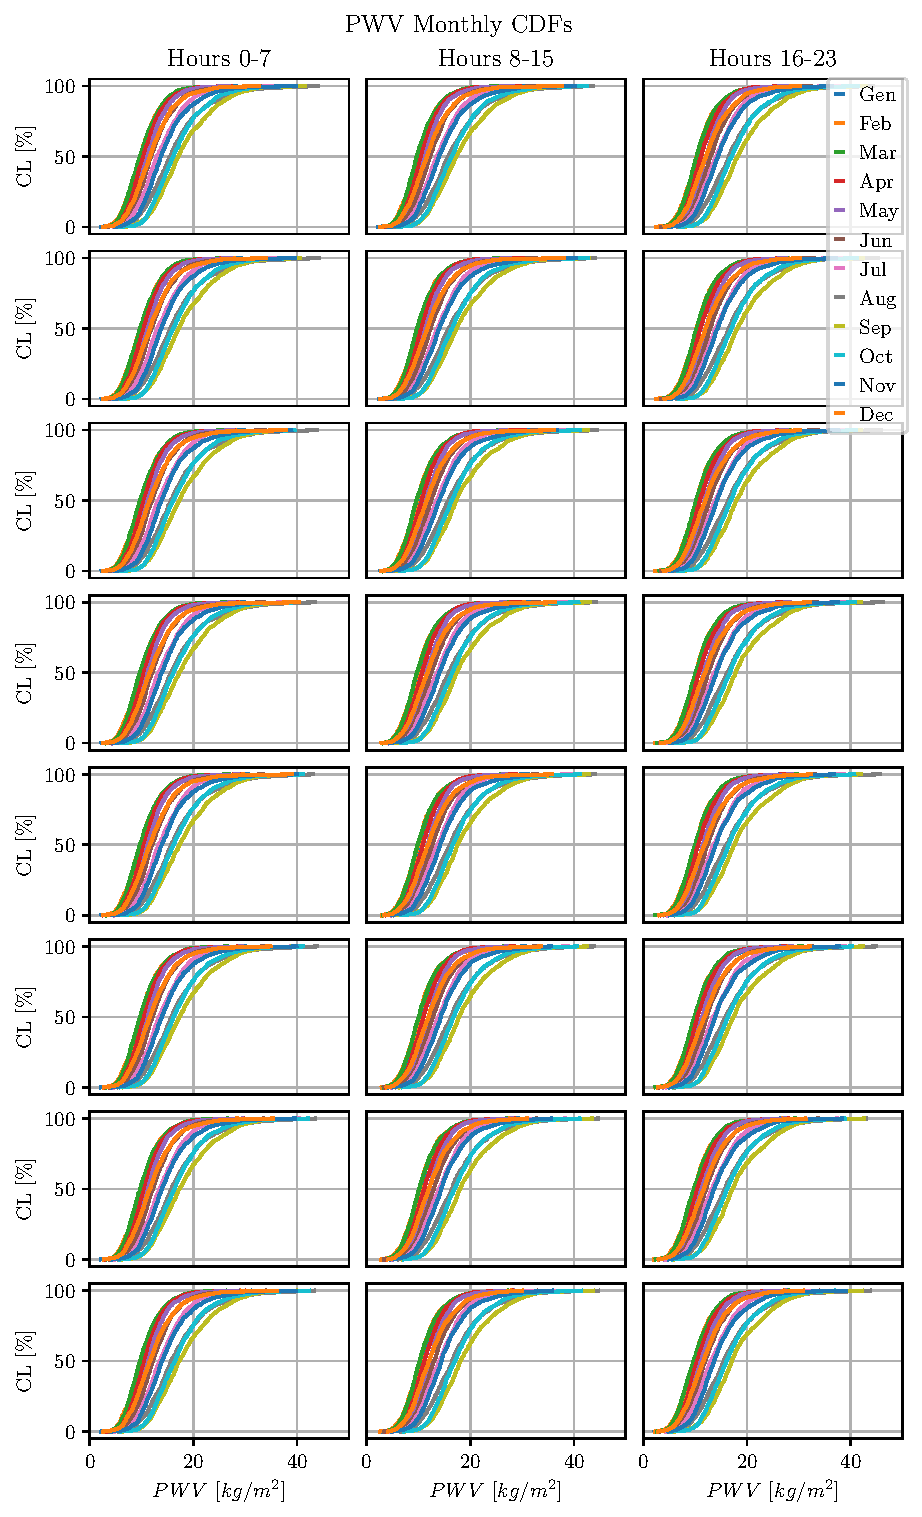
\includegraphics[width=0.76\textwidth]{PWV_Monthly_CDFs}
        \caption{Cumulative distribution functions for every hour of a
        typical day of each month of the year for the PWD parameter at Pico
        del Teide. Months are represented using different colors and
        probability is expressed in terms of \emph{confidence level}.}
        \label{fig:pwv_monthly_cdfs}
\end{figure}

CDFs data have been subsequently decimated and saved in \texttt{.fits} file
format. We will refer to this representation simply as the \emph{CDFs
\texttt{.fits} file}. The structure of the latter
follows:

\begin{Verbatim}[fontsize=\scriptsize]
No.    Name      Ver    Type      Cards   Dimensions   Format
  0  PRIMARY       1 PrimaryHDU       4   ()
  1                1 BinTableHDU     30   24R x 8C   [101D, 101D, 101D, 101D, 101D, 101D, 101D, 101D]
  2                1 BinTableHDU     30   24R x 8C   [101D, 101D, 101D, 101D, 101D, 101D, 101D, 101D]
  3                1 BinTableHDU     30   24R x 8C   [101D, 101D, 101D, 101D, 101D, 101D, 101D, 101D]
  4                1 BinTableHDU     30   24R x 8C   [101D, 101D, 101D, 101D, 101D, 101D, 101D, 101D]
  5                1 BinTableHDU     30   24R x 8C   [101D, 101D, 101D, 101D, 101D, 101D, 101D, 101D]
  6                1 BinTableHDU     30   24R x 8C   [101D, 101D, 101D, 101D, 101D, 101D, 101D, 101D]
  7                1 BinTableHDU     30   24R x 8C   [101D, 101D, 101D, 101D, 101D, 101D, 101D, 101D]
  8                1 BinTableHDU     30   24R x 8C   [101D, 101D, 101D, 101D, 101D, 101D, 101D, 101D]
  9                1 BinTableHDU     30   24R x 8C   [101D, 101D, 101D, 101D, 101D, 101D, 101D, 101D]
 10                1 BinTableHDU     30   24R x 8C   [101D, 101D, 101D, 101D, 101D, 101D, 101D, 101D]
 11                1 BinTableHDU     30   24R x 8C   [101D, 101D, 101D, 101D, 101D, 101D, 101D, 101D]
 12                1 BinTableHDU     30   24R x 8C   [101D, 101D, 101D, 101D, 101D, 101D, 101D, 101D]
None
\end{Verbatim}

The CDFs \texttt{.fits} file includes \num{12} $24 \times 8$ binary tables:
one table for each month of the year. As an example, header information for
the January table is shown:

\begin{Verbatim}
XTENSION= 'BINTABLE'           / binary table extension
BITPIX  =                    8 / array data type
NAXIS   =                    2 / number of array dimensions
NAXIS1  =                 6464 / length of dimension 1
NAXIS2  =                   24 / length of dimension 2
PCOUNT  =                    0 / number of group parameters
GCOUNT  =                    1 / number of groups
TFIELDS =                    8 / number of table fields
TTYPE1  = 'TQL     '
TFORM1  = '101D    '
TTYPE2  = 'TQI     '
TFORM2  = '101D    '
TTYPE3  = 'TQV     '
TFORM3  = '101D    '
TTYPE4  = 'TS      '
TFORM4  = '101D    '
TTYPE5  = 'PS      '
TFORM5  = '101D    '
TTYPE6  = 'T10M    '
TFORM6  = '101D    '
TTYPE7  = 'V10M    '
TFORM7  = '101D    '
TTYPE8  = 'U10M    '
TFORM8  = '101D    '
MONTH   =                    0
PROBSTRT=                  0.0
PROBSTOP=                  1.0
PROBSTEP=                 0.01
NSTEP   =                  101
SOURCE  = 'ERA5 data from 1979 to 2020'
\end{Verbatim}

As can be observed, every binary table has \num{8} columns, one for each
relevant meteorological parameter. Every column is a matrix of $101 \times
24$ double size floating point ordered values, one data for each
percentile, representing a discretization of a CDF function.  The CDFs
\texttt{.fits} file is rather light (\SI{\sim 2}{\mega\byte}) and can be
employed by instrumental simulations frameworks such as
\emph{TOAST}\footnote{\url{https://github.com/hpc4cmb/toast}},
\emph{QUBIC\_Soft} \footnote{\url{https://github.com/qubicsoft/qubic}} and
\emph{Stripeline}
\footnote{\url{https://github.com/lspestrip/Stripeline.jl}} in order to
produce simulations ground-based experiments observations. Furthermore,
this method can be adapted for use at any site.

\section{The Seasonal Matrices}

The atmospheric statistical picture constitutes an effective tool to
predict seasonal variations of the parameters of interest. By evaluating
cumulative distribution functions at different \emph{confidence levels}
(CL), different expectation values for the meteorological parameters can be
obtained. \autoref{fig:teide_seasonal_matrices_vertical} shows heatmap
representations of the median seasonal variations of PWV, $T_s$ and $P_s$,
which have been obtained evaluating the respective CDFs at the
\SI{50}{\percent} confidence level. Change in colour along a row
or a column represents daily or yearly variations of the meteorological
parameters, respectively. We refer to these map representations of our
realization of the atmosphere as the \emph{seasonal matrices}. Median
is a particularly appropriate estimator for atmospheric parameters, because
rare bad weather events, such as heavy rain, snow and wind guts, which
fall in the tails of the probability distribution, do not have an excessive
weight on the expectation value.


\begin{figure}
        \centering
        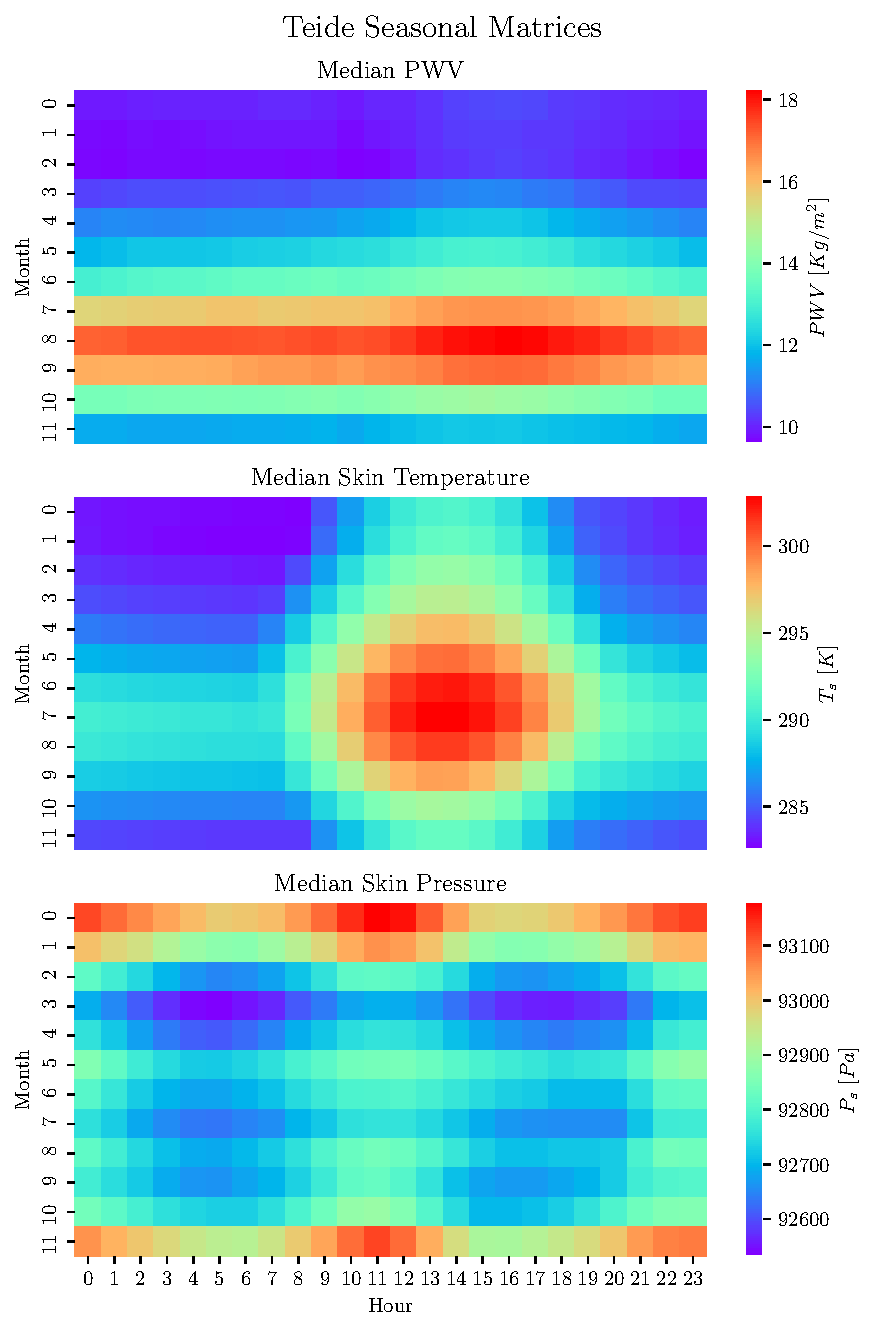
\includegraphics[width=0.91\textwidth]{Teide_Seasonal_Matrices_vertical}
        \caption{Seasonal Matrices for PWV, skin temperature and surface
        pressure at Pico del Teide.}
        \label{fig:teide_seasonal_matrices_vertical}
\end{figure}

